Il modello di sviluppo adottato si ispira a quello \textbf{incrementale} secondo ISO/IEC 12207:1995, cosicché possano essere garantite la qualità$^*$ e la conformità attese durante lo svolgimento del progetto$^*$.

\subsection{Il modello di sviluppo}
Nel modello incrementale, il numero di incrementi viene pianificato in base ai requisiti identificati durante l'analisi. Essi vengono ordinati in base alla loro priorità che viene determinata in base all'importanza strategica.\\
Dopo di che, si passa alla suddivisione dei requisiti nei vari incrementi. Chiaramente, quelli più incombenti, ovvero quelli a priorità più alta, saranno assegnati ai primi incrementi dell'iterazione. In tal modo, il prodotto viene consegnato al committente incrementalmente tramite Proof of Concept$^*$.\\
Durante gli incrementi, non può essere aggiunto o modificato alcun requisito. Se ciò dovesse essere necessario, il requisito verrà aggiunto a quelli dell'incremento successivo. Una volta completato il suo sviluppo, esso viene aggiunto al prodotto.\\
La scelta del modello incrementale aiuta la definizione dei requisiti, che sono il punto critico del progetto. Infatti, la proponente non ha posto vincoli particolarmente stringenti sulle tecnologie da impiegare: ciò da un lato permette una certa libertà di azione al team, dall'altro non permette un'identificazione veloce dei requisiti tecnologici. Il modello incrementale prevede nell'ordine l'analisi dei requisiti del sistema, la progettazione architetturale del sistema, l'analisi dei requisiti software e, infine, la progettazione architetturale del software. Lo svolgimento di attività di progettazione prima del completamento dell'analisi permetterà la determinazione dei requisiti tecnologici non ancora identificati.

\subsection{Organizzazione del modello}
Il modello adottato è composto da 4 fasi principali:
\subsubsection{Fase 1: Avvio e Analisi dei requisiti (2018-12-04 - 2019-01-21)} 
Questa fase si suddivide in 2 periodi: \\
\textbf{Periodo di avvio (2018-12-4 - 2018-12-17):} 
durante questa fase, il gruppo si impegna nella ricerca delle tecnologie utili per lo \textit{StudioDiFattibilità\_v1.0.0}. Inoltre si procede con una prima normazione che sarà presente nel documento \textit{NormeDiProgetto\_v1.0.0} e per poter svolgere i processi in maniera ordinata e regolamentata nel \textit{PianoDiProgetto\_v1.0.0} sarà presente la pianificazione di ogni attività.\\
\textbf{Periodo di analisi dei Requisiti (2018-12-18 - 2019-01-14):} nel \textit{PianoDiQualifica\_v1.0.0} saranno specificati dopo essere stati individuati, i vari metodi per garantire qualità al prodotto e successivamente si passa con l'analisi dei requisiti del sistema.

\subsubsection{Fase 2: Progettazione della base tecnologica (2019-01-22 - 2019-03-15)}
Vengono eseguiti gli incrementi in base agli scostamenti rilevati nella Revisione dei Requisiti.
Vengono poi studiate, analizzate e normate le scelte tecnologiche, i framework e librerie utili per sviluppare il prodotto. Una volta individuate, si progetta e si esegue la codifica del Proof of Concept.\\

\subsubsection{Fase 3: Progettazione di dettaglio e codifica (2019-03-16 - 2019-04-19)}
Vengono eseguiti gli incrementi in base agli scostamenti rilevati nella Revisione di Progettazione.
Si procede poi con la realizzazione del \textit{Product Baseline} che descrive l'architettura del prodotto.
Sono previsti tre incrementi composti ognuno da attività di progettazione, codifica e verifica.
Inoltre verrà redatto il \textit{ManualeUtente\_v0.1.0}.\\

\subsubsection{Fase 4: Validazione e collaudo (2019-04-20 - 2019-05-17)}
Vengono eseguiti gli incrementi in base agli scostamenti rilevati nella Revisione di Qualifica.
Si effettueranno i test di qualifica. Nel caso in cui tali test abbiano esito negativo è possibile correre ai ripari tramite attività di progettazione e codifica. Una volta che il test di qualifica ha esito positivo, è possibile procedere al collaudo.
Infine, il prodotto è pronto per essere consegnato.

\subsection{Attività}
Ogni incremento prevede delle attività ed è diviso nelle seguenti fasi:
\begin{itemize}
	\item Si assegnano i task ai vari componenti del gruppo;
	\item Vengono completati i compiti assegnati entro 3-7 giorni;
	\item Si effettuano le verifiche sui prodotti completati e valutati se ritenuti soddisfacenti o meno. Nel caso in cui il risultato sia soddisfacente, l'attività è considerata conclusa, altrimenti lo sviluppatore dovrà correggere dove indicato entro 3 giorni e procedere alla verifica del prodotto modificato.
\end{itemize}
Il numero massimo di incrementi svolti su un prodotto dipende dalla complessità del compito e dal termine della fase a cui l'attività è stata assegnata.

\begin{figure}[h]
	\centering
	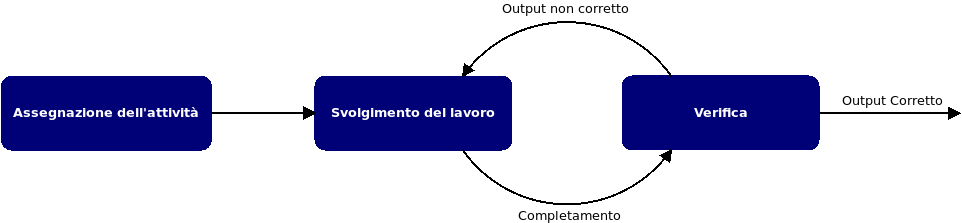
\includegraphics[scale=0.45]{images/Model/activity.png}
	\caption{Ciclo di un'attività}
\end{figure}
